%!TEX program = xelatex
\documentclass[a4paper,UTF8]{ctexart}
\usepackage[unicode=true,colorlinks,breaklinks=true,urlcolor=blue,linkcolor=blue,bookmarksnumbered=true]{hyperref}
\usepackage{latexsym,amssymb,amsmath,amsbsy,amsopn,amstext,amsthm,amsxtra,color,multicol,bm,calc,ifpdf}
\usepackage{graphicx}
\usepackage{diagbox}   % 绘制表格斜线
\usepackage{enumerate}
\usepackage{epstopdf}
\usepackage{fancyhdr}
\usepackage{subfigure}
\usepackage{listings}
\usepackage{multirow}
\usepackage{makeidx}
\usepackage{xcolor} 
\usepackage{fontspec}                            % 建立索引宏包
\graphicspath{{figures/}}  % 设置图片搜索路径
\theoremstyle{plain} \newtheorem{theorem}{定理}[section]
\theoremstyle{plain} \newtheorem{definition}{定义}[section]
\theoremstyle{plain} \newtheorem{lemma}{引理}[section]
\theoremstyle{plain} \newtheorem{proposition}{命题}[section]
\theoremstyle{plain} \newtheorem{example}{例}[section]
\theoremstyle{plain} \newtheorem{remark}{注}[section]
\theoremstyle{plain} \newtheorem{corollary}{推论}[section]
\newfontfamily\courier{Courier New}
\lstset{linewidth=1.1\textwidth,
        numbers=left, %设置行号位置 
        basicstyle=\small\courier,
        numberstyle=\tiny\courier, %设置行号大小  
        keywordstyle=\color{blue}\courier, %设置关键字颜色  
        %identifierstyle=\bf,
        commentstyle=\it\color[cmyk]{1,0,1,0}\courier, %设置注释颜色 
        stringstyle=\it\color[RGB]{128,0,0}\courier,
        %framexleftmargin=10mm,
        frame=single, %设置边框格式  
        backgroundcolor=\color[RGB]{245,245,244},
        %escapeinside=``, %逃逸字符(1左面的键),用于显示中文  
        breaklines, %自动折行  
        extendedchars=false, %解决代码跨页时,章节标题,页眉等汉字不显示的问题  
        xleftmargin=2em,xrightmargin=2em, aboveskip=1em, %设置边距  
        tabsize=4, %设置tab空格数  
        showspaces=false %不显示空格  
        basicstyle=\small\courier
       }  
\newenvironment{mysolution}{{\color{blue} 解}: }{{\color{magenta}\qed}}
\newcommand\diff{\,{\mathrm d}} % 定义微分 d
\newcommand{\p}[3]{\frac{\partial^{#1}#2}{\partial{#3}^{#1}}}  % 定义求偏导算子
\newcommand{\ucite}[1]{\textsuperscript{\cite{#1}}}  % 参考文献引用: 上标用 \ucite{ }, 文中用 \cite{ }

\begin{document}
\title{

\includegraphics[width=0.65\textwidth]{onepiece.pdf}\\
\vspace{2em}
\textbf{Logistic 回归学习笔记}}
\author{\emph{李向阳} \quad {\color{blue} d1142845997@gmail.com}
}
\date{}


\maketitle
\thispagestyle{empty}

\newpage


\tableofcontents

\newpage

\section{基本 Logistic 回归}

\subsection{数据集}
在二分类问题中, 我们的样本是$\{\bm{x},y\}$, 其中$y$是$0$或者$1$, $y = 1$表示正类, $y = 0$表示负类(也有些文献中用$y = \pm 1$区分正负类), 而$\bm{x}$表示样本的特征, 设有$n$个特征, 即$\bm{x} = (x_{1}, x_{2}, \cdots, x_{n})^{T}$, 因此我们也可以将样本表示为$\{ x_{1}, \cdots, x_{n}, y \}$, 我们的期待是由这$n$个样本特征来预测样本的类别. 设训练集有$m$个样本, 即$\{\bm{x}^{(i)}, y^{(i)}\}, i = 1,2,\cdots,m$, 其中
\begin{equation*}
\bm{x}^{(i)} = (x_{1}^{(i)}, x_{2}^{(i)}, \cdots, x_{n}^{(i)})^{T},i = 1,2,\cdots,m
\end{equation*}

这里要注意记号的不同, 也有些文献中把粗体的$\bm{x}$用$\mathbf{x}$来表示, 这里我们仍将粗体倾斜.

关于记号, 这里要多说一点, 这篇文章中我用粗体的$\bm{x}$表示样本, 它有$n$个分量, 分量用下标表示, 即有$\bm{x} = (x_{1}, x_{2}, \cdots, x_{n})^{T}$, 用上标表示具体的样本, 即$\bm{x}^{(i)}$表示第$i$个样本, 并设总共有$m$个样本. 采用这样的记号, 个人觉得比采用双下标要好一些, 但推导时还是略显麻烦, 因此有些文献中会采用这样的记号: 用粗体的$\bm{x}$表示样本, 同时用带下标$i$的$\bm{x}_{i}$表示第$i$个样本, 注意$\bm{x}_{i}$实际上有$n$个分量, 但为了推导方便并不写出, 直接理解为带$n$个分量的向量即可(不过要加粗, 有些文档中甚至不加粗, 这很不好), 然后设样本个数为$N$. 这也是一种常见的记号.

\subsection{基本模型}
所谓 Logistic 回归模型, 也就是假设样本$\bm{x}$属于正类或者说对应的$y = 1$的概率可以通过 sigmoid 函数来表示:
\begin{equation}\label{eq:logit-model}
\begin{split}
P(y = 1 | \bm{x}; \bm{\theta}) & = \sigma(\bm{\theta}^{T} \bm{x}) = h_{\bm{\theta}}(\bm{x}) = \frac{1}{1 + \exp(- \bm{\theta}^{T} \bm{x})} \\
& = \frac{1}{1 + \exp(-(\theta_{0} + \theta_{1} x_{1} + \cdots + \theta_{n} x_{n}))}
\end{split}
\end{equation}

\begin{figure}[!htb]
	\centering
	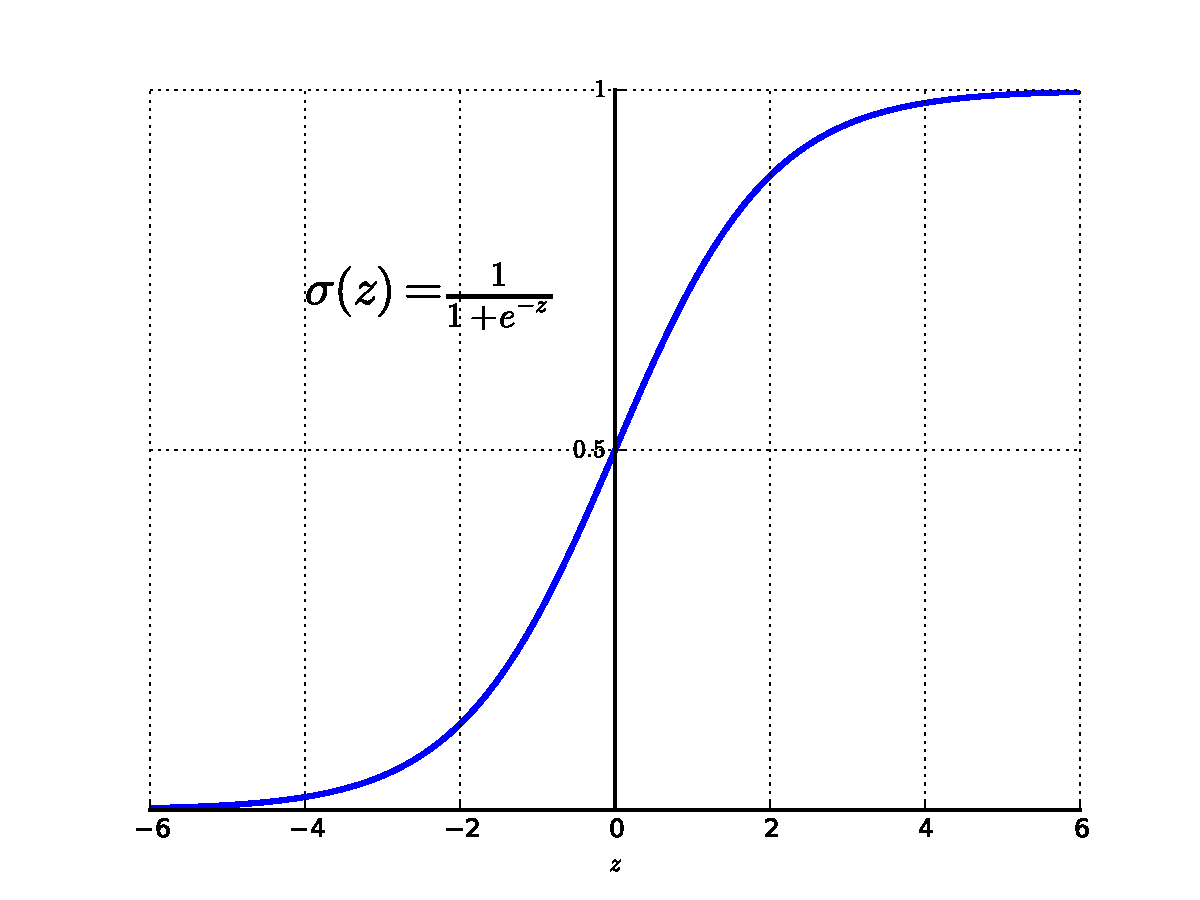
\includegraphics[width=0.80\textwidth]{sigmoid_fig.pdf}
	\caption{sigmoid函数图像}
\end{figure}

注意这里为了记号的方便, 引入$x_{0} = 1$, 即有$\bm{x} = (x_{0}, x_{1}, \cdots, x_{n})^{T}$, 而$\bm{\theta} = (\theta_{0}, \theta_{1}, \cdots, \theta_{n})^{T}$, $\bm{\theta}$是模型参数, 或者称为回归系数.

以上的想法是对样本属于正类的概率进行建模, 也就是给样本$\bm{x} = (x_1, x_2, \cdots, x_n)^{T}$的每个特征赋予一个“权重”(可正可负), 即$\theta_1, \theta_2, \cdots, \theta_n$, 然后计算这些特征的加权值$\theta_0 + \theta_1 x_1 + \theta_2 x_2 + \cdots + \theta_n x_n$, 其中$\theta_0$为常数. 为了使加权值能够转化为概率, 上面考虑了 sigmoid 函数, 由此导出了 Logistic 回归模型.

此外, 我们还可以从对数几率的角度来得到 Logistic 回归模型. 一个事件的几率是指其发生的概率与不发生的概率的比值. 如果事件发生的概率是$p$, 根据定义, 该事件的几率是$\dfrac{p}{1 - p}$, 其对数几率或 logit 函数是
\begin{equation}
\mathrm{logit}(p) = \log \frac{p}{1 - p}
\end{equation}

假设样本属于正类的对数几率是样本输入特征$\bm{x}$的线性函数, 即
\begin{equation}
\log \frac{P(y = 1 | \bm{x})}{1 - P(y = 1 | \bm{x})} = \bm{\theta}^{T} \bm{x} = \theta_0 + \theta_1 x_ 1 + \cdots + \theta_n x_n
\end{equation}

化简可得式(\ref{eq:logit-model}), 同样得到了 Logistic 回归模型. 也就是说, 对几率做了对数变换以后, 成了线性模型. 事实上, Logistic 回归本身就是一种广义线性模型, 也可以从广义线性模型的角度推导出来(可参考 Andrew Ng 的课件).

\begin{remark}
上面已经指出, Logistic 回归的模型是
\begin{equation*}
p(y = 1 | \bm{x}) = \frac{1}{1 + \exp(- \bm{\theta}^T \bm{x}}), \ln \frac{p}{1 - p} = \bm{\theta}^T \bm{x}
\end{equation*}

Logistic 模型也称之为 Logit 模型, 与之类似的有一个模型, 称为 Probit 模型, 其假设是
\begin{equation*}
p(y = 1 | \bm{x}) = \Phi (\bm{\theta}^T \bm{x}), \Phi^{-1}(p) = \bm{\theta}^T \bm{x}
\end{equation*}

其中$\Phi(\cdot)$是标准正态分布的累积分布函数, 由此可以看出二者的不同. 即 Logit 模型是借助函数$\Phi(\cdot)$将$\bm{\theta}^T \bm{x}$转化为了概率值, 而 Logistic 模型是借助 sigmoid 函数将$\bm{\theta}^T \bm{x}$转化为了概率值. 要注意区分. 不过, 由于只是转化函数不同, 因此二者的参数估计是很类似的. 当然, 对于 Probit regression model, 更常用的是借助 EM 算法估计其参数.

\end{remark}

Logistic 回归的任务便是利用训练样本得到$\bm{\theta}$的参数估计, 不妨记为$\hat{\bm{\theta}}$, 于是得到预测模型为
\begin{equation*}
P(y = 1 | \bm{x}) = \frac{1}{1 + \exp (- \hat{\bm{\theta}}^{T} \bm{x})}
\end{equation*}

当得到一个新的样本$\bm{x}^{(0)}$后, 代入上式可计算该样本属于正类的概率, 若其值大于$0.5$, 我们将其归为正类, 反之则归为负类.


\subsection{参数估计}
这里我们采用最大似然估计方法. 注意在机器学习的一般框架中, 为了估计模型参数, 常常构造称为代价函数(cost function)或者损失函数(loss function)的东西, 然后将其极小化得到参数的估计, 比如将似然函数取负号作为代价函数, 二者的实质是一样的
.

由定义可知, 对于样本$\bm{x}$, 其为正类和负类的概率分别为
\begin{equation*}
P(y = 1 | \bm{x}; \bm{\theta}) = h_{\bm{\theta}}(\bm{x}),  P(y = 0 | \bm{x}; \bm{\theta}) = 1 - h_{\bm{\theta}}(\bm{x})
\end{equation*}

实际上这是一个$0-1$分布(伯努利分布), 其概率函数为
\begin{equation*}
p(y | \bm{x}; \bm{\theta}) = (h_{\bm{\theta}}(\bm{x}))^{y} (1 - h_{\bm{\theta}}(\bm{x}))^{1 - y}
\end{equation*}

由于假定$m$个训练样本独立同分布, 故似然函数为
\begin{align*}
L(\bm{\theta}) & = \prod_{i=1}^{m} p(y^{(i)} | \bm{x}^{(i)}; \bm{\theta}) \\
& = \prod_{i=1}^{m} (h_{\bm{\theta}}(\bm{x}^{(i)}))^{y^{(i)}} (1 - h_{\bm{\theta}}(\bm{x}^{(i)}))^{1 - y^{(i)}}
\end{align*}

其对数似然函数为
\begin{equation*}
l(\bm{\theta}) = \log L(\bm{\theta}) = \sum_{i=1}^{m} \left( y^{(i)} \log h_{\bm{\theta}}(\bm{x}^{(i)}) + (1 - y^{(i)}) \log (1 - h_{\bm{\theta}}(\bm{x}^{(i)})) \right)
\end{equation*}

最大似然估计就是求使$l(\bm{\theta})$取得最大值时的$\bm{\theta}$, 此时如果用求导的办法求最大值的话, 会发现是无法求得解析解的. 当然, 我们可以用优化中的许多方法进行数值求解.

现在, 我们转向机器学习的框架来考虑参数估计. 构造关于参数$\bm{\theta}$的代价函数$J(\bm{\theta})$, 在这里, 我们将对数似然函数取个符号, 然后再除以常数$m$(即为训练样本个数), 即
\begin{equation*}
J(\bm{\theta}) = - \frac{1}{m} l(\bm{\theta}) = - \frac{1}{m} \sum_{i=1}^{m} \left[ y^{(i)} \log h_{\bm{\theta}}(\bm{x}^{(i)}) + (1 - y^{(i)}) \log (1 - h_{\bm{\theta}}(\bm{x}^{(i)})) \right]
\end{equation*}

因为乘了一个负的系数$-1 / m$, 所以极小化$J(\bm{\theta})$与最大化$l(\bm{\theta})$是等价的.

此外, 代价函数还可由下式定义:
\begin{equation*}
J(\bm{\theta}) = \frac{1}{m} \mathrm{Cost}(h_{\bm{\theta}}(\bm{x}),y)
\end{equation*}

其中$\mathrm{Cost}(h_{\bm{\theta}}(\bm{x}), y)$为对数损失函数, 
$$
\mathrm{Cost}(h_{\bm{\theta}}(\bm{x}), y) = 
\begin{cases}
-\log(h_{\bm{\theta}}(\bm{x}))  , & y = 1 \\
-\log(1 - h_{\bm{\theta}}(\bm{x})) , & y = 0
\end{cases}
$$

由此得到
\begin{equation*}
J(\bm{\theta}) = - \frac{1}{m} \sum_{i=1}^{m} \left[ y^{(i)} \log h_{\bm{\theta}}(\bm{x}^{(i)}) + (1 - y^{(i)}) \log (1 - h_{\bm{\theta}}(\bm{x}^{(i)})) \right]
\end{equation*}

\begin{remark}
对数损失函数的一般形式为(可参考\url{http://www.csuldw.com/2016/03/26/2016-03-26-loss-function/})
\begin{equation*}
L(y, p(y | \bm{x})) = - \log p(y | \bm{x})
\end{equation*}

\end{remark}


\begin{remark}
我们可以对损失函数做进一步的化简, 即有(先略去常数因子$-1 / m$, 参考: \url{http://blog.csdn.net/zouxy09/article/details/20319673})
\begin{align*}
l(\bm{\theta}) & = \sum_{i=1}^{m} \left[y^{(i)} \log h_{\bm{\theta}}(\bm{x}^{(i)}) + (1-y^{(i)}) \log (1-h_{\bm{\theta}}(\bm{x}^{(i)})) \right] \\ 
& = \sum_{i=1}^{m} \left[y^{(i)} \log p(y^{(i)} = 1 | \bm{x}^{(i)}) + (1-y^{(i)}) \log (1 - p(y^{(i)} = 1 | \bm{x}^{(i)})) \right] \\
& = \sum_{i=1}^{m} y^{(i)} \log \frac{p(y^{(i)} = 1 | \bm{x}^{(i)})}{1 - p(y^{(i)} = 1 | \bm{x}^{(i)})} + \sum_{i=1}^{m} \log (1 - p(y^{(i)} = 1 | \bm{x}^{(i)})) \\ 
& = \sum_{i=1}^{m} y^{(i)} \cdot \bm{\theta}^{T} \bm{x}^{(i)} + \sum_{i=1}^{m} \log \frac{1}{1 + \exp (\bm{\theta}^{T} \bm{x}^{(i)})} \\ 
& = \sum_{i=1}^{m} y^{(i)} \cdot \bm{\theta}^{T} \bm{x}^{(i)} - \sum_{i=1}^{m} \log (1 + \exp (\bm{\theta}^{T} \bm{x}^{(i)}))
\end{align*}

由此可得
\begin{equation}\label{simplifyloss}
J(\bm{\theta}) = \frac{1}{m} \left[ \sum_{i=1}^{m} \log (1 + \exp (\bm{\theta}^{T} \bm{x}^{(i)})) - \sum_{i=1}^{m} y^{(i)} \cdot \bm{\theta}^{T} \bm{x}^{(i)} \right]
\end{equation}

此时可直接对$\bm{\theta}$求导(下面又用了复杂的方法推导)
\begin{align*}
\p{}{J(\bm{\theta})}{\bm{\theta}} & = \frac{1}{m} \left[ \sum_{i=1}^{m} \frac{\exp(\bm{\theta}^{T} \bm{x}^{(i)})}{1 + \exp(\bm{\theta}^{T} \bm{x}^{(i)})} \bm{x}^{(i)} - \sum_{i=1}^{m} y^{(i)} \bm{x}^{(i)} \right] \\ 
& = \frac{1}{m} \sum_{i=1}^{m} \left( \sigma(\bm{\theta}^{T} \bm{x}^{(i)}) - y^{(i)} \right) \bm{x}^{(i)}
\end{align*}

如果令导数为$0$, 会发现是无法得到解析解的, 所以需要用下面的迭代法进行计算.

\end{remark}


\begin{remark}
以上的讨论和损失函数都是针对样本类别标签$y$取值为$1$或$0$的情形, 有些资料中使用的是$\pm 1$来区分正负类, 即$y$的取值为$1$或$-1$, 此时的表达方式略有不同. 这里稍微提一下.

如果用$y = \pm 1$区分正负类, 那么样本的概率可以表示为
\begin{equation*}
p(y | \bm{x}; \bm{\theta}) = \frac{1}{1 + \exp (- y \cdot \bm{\theta}^T \bm{x})} = \frac{1}{1 + \exp (- y f(\bm{x}))}
\end{equation*}

其中$f(\bm{x}) = \bm{\theta}^T \bm{x}$.

类似的, 似然函数为
\begin{align*}
l(\bm{\theta}) & = \log \prod_{i=1}^{m} p(y^{(i)}|\bm{x}^{(i)};\bm{\theta}) \\ 
& = \sum_{i=1}^{m} \log p(y^{(i)}|\bm{x}^{(i)};\bm{\theta}) \\ 
& = \sum_{i=1}^{m} - \log (1 + \exp (- y^{(i)} f(\bm{x}^{(i)})))
\end{align*}

因此损失函数为
\begin{equation*}
J(\bm{\theta}) = -\frac{1}{m} l(\bm{\theta}) = \frac{1}{m} \sum_{i=1}^{m} \log (1 + \exp (- y^{(i)} f(\bm{x}^{(i)})))
\end{equation*}

当然, 我们也可以直接从损失函数的角度来得到这个表达式(仍可参考: \url{http://www.csuldw.com/2016/03/26/2016-03-26-loss-function/}), 事实上, 在 Logistic 回归中, 我们采用的是对数损失函数
\begin{equation*}
L(y, p(y | \bm{x})) = - \log p(y | \bm{x})
\end{equation*}

由于
\begin{equation*}
p(y | \bm{x}) = \frac{1}{1 + \exp (- y f(\bm{x}))}
\end{equation*}

因此损失函数为
\begin{equation*}
L(y, p(y | \bm{x})) = \log (1 + \exp (- y f(\bm{x})))
\end{equation*}

整个样本集合的损失函数为
\begin{equation*}
J(\bm{\theta}) = \frac{1}{m} \sum_{i=1}^{m} L(y^{(i)}, p(y^{(i)} | \bm{x}^{(i)})) = \frac{1}{m} \sum_{i=1}^{m} \log (1 + \exp (- y^{(i)} f(\bm{x}^{(i)})))
\end{equation*}

即我们直接从损失函数的角度也得到了$J(\bm{\theta})$的表达式.

这里额外提一点, 就是这里的$J(\bm{\theta})$的表达式与上面(\ref{simplifyloss})的表达式结果相同吗?

事实上是一样的, (\ref{simplifyloss})式可化为
\begin{align*}
J(\bm{\theta}) & = \frac{1}{m} \left[ \sum_{i=1}^{m} \log (1 + \exp (f(\bm{x}^{(i)}))) - \sum_{i=1}^{m} y^{(i)} f(\bm{x}^{(i)}) \right] \\ 
& = \frac{1}{m} \sum_{i=1}^{m} \log \left[ (1 + \exp (f(\bm{x}^{(i)}))) \cdot \exp (- y^{(i)} f(\bm{x}^{(i)})) \right]
\end{align*}

因此, 在(\ref{simplifyloss})里面令$y^{(i)} = 1$与现在令里面令$y^{(i)} = 1$的结果相同, 在在(\ref{simplifyloss})里面令$y^{(i)} = 0$与现在令里面令$y^{(i)} = -1$的结果也相同. 也就是说类标记$y$用$1, 0$区分和用$\pm 1$区分是几乎一样的.

\end{remark}

接下来我们需要求$J(\bm{\theta})$的最小值, 可以采用梯度下降法(即最速下降法)、共轭梯度法、拟牛顿法等优化方法. 这里以梯度下降法为例进行分析, 其迭代更新公式为
\begin{equation*}
\bm{\theta} : = \bm{\theta} - \alpha \cdot \nabla J(\bm{\theta})
\end{equation*}

其中$\alpha$为步长, $\bm{\theta} = (\theta_{0}, \theta_{1}, \cdots, \theta_{n})^{T}$, 写成分量形式即为
\begin{equation*}
\theta_{j} : = \theta_{j} - \alpha \cdot \p{}{J(\bm{\theta})}{\theta_{j}}
\end{equation*}

计算可得
\begin{equation*}
\p{}{J(\bm{\theta})}{\theta_{j}} = \frac{1}{m} \sum_{i=1}^{m} (h_{\bm{\theta}}(\bm{x}^{(i)}) - y^{(i)}) x_{j}^{(i)}
\end{equation*}

下面说一下计算方法. 为了记号的简便, 我们用$h'_{\bm{\theta}}(\bm{x}^{(i)})$表示$h_{\bm{\theta}}(\bm{x}^{(i)})$对$\theta_{j}$求偏导, $j = 0,1,\cdots,n$, 注意到
\begin{equation*}
h_{\bm{\theta}}(\bm{x}^{(i)}) = \frac{1}{1 + \exp (- \bm{\theta}^{T} \bm{x}^{(i)})} = \frac{1}{1 + \exp (-(\theta_{0} x_{0}^{(i)} + \theta_{1} x_{1}^{(i)} + \cdots + \theta_{n} x_{n}^{(i)}))}
\end{equation*}

运用复合函数求导法则可得
\begin{align*}
h'_{\bm{\theta}}(\bm{x}^{(i)}) & = \p{}{h_{\bm{\theta}}(\bm{x}^{(i)})}{\theta_{j}} = - h^{2}_{\bm{\theta}}(\bm{x}^{(i)}) \cdot \exp (-\bm{\theta}^{T} \bm{x}^{(i)}) \cdot (- x_{j}^{(i)}) \\
& = h^{2}_{\bm{\theta}}(\bm{x}^{(i)}) \left( \frac{1}{h_{\bm{\theta}}(\bm{x}^{(i)})} - 1 \right) x_{j}^{(i)} \\
& = h_{\bm{\theta}}(\bm{x}^{(i)}) (1 - h_{\bm{\theta}}(\bm{x}^{(i)})) x_{j}^{(i)}
\end{align*}

其实自己在下面推导时是可以暂时把上标$i$忽略掉的, 此外还可以得到(求梯度与求导很相似)
\begin{equation*}
\nabla h_{\bm{\theta}}(\bm{x}^{(i)}) = h_{\bm{\theta}}(\bm{x}^{(i)}) (1 - h_{\bm{\theta}}(\bm{x}^{(i)})) \bm{x}^{(i)}
\end{equation*}

另一方面
\begin{align*}
\p{}{J(\bm{\theta})}{\theta_{j}} & = - \frac{1}{m} \left( \sum_{i=1}^{m} y^{(i)} \cdot \frac{h'_{\bm{\theta}}(\bm{x}^{(i)})}{h_{\bm{\theta}}(\bm{x}^{(i)})} + (1 - y^{(i)}) \cdot \frac{-h'_{\bm{\theta}}(\bm{x}^{(i)})}{1 - h_{\bm{\theta}}(\bm{x}^{(i)})} \right) \\
& = -\frac{1}{m} \left( \sum_{i=1}^{m} \frac{y^{(i)}(1 - h_{\bm{\theta}}(\bm{x}^{(i)})) h'_{\bm{\theta}}(\bm{x}^{(i)}) + (y^{(i)} - 1) h_{\bm{\theta}}(\bm{x}^{(i)}) h'_{\bm{\theta}}(\bm{x}^{(i)})}{h_{\bm{\theta}}(\bm{x}^{(i)}) (1 - h_{\bm{\theta}}(\bm{x}^{(i)}))}  \right) \\
& = - \frac{1}{m} \left( \sum_{i=1}^{m} \frac{y^{(i)} h'_{\bm{\theta}}(\bm{x}^{(i)}) - y^{(i)} h_{\bm{\theta}} (\bm{x}^{(i)}) h'_{\bm{\theta}}(\bm{x}^{(i)}) + y^{(i)} h_{\bm{\theta}}(\bm{x}^{(i)})h'_{\bm{\theta}} (\bm{x}^{(i)}) - h_{\bm{\theta}} (\bm{x}^{(i)}) h'_{\bm{\theta}}(\bm{x}^{(i)}) } {h_{\bm{\theta}}(\bm{x}^{(i)}) (1 - h_{\bm{\theta}} (\bm{x}^{(i)}))} \right) \\
& = - \frac{1}{m} \left( \sum_{i=1}^{m} \frac{(y^{(i)} - h_{\bm{\theta}}(\bm{x}^{(i)}) ) \cdot h'_{\bm{\theta}} (\bm{x}^{(i)})} {h_{\bm{\theta}} (\bm{x}^{(i)}) (1 - h_{\bm{\theta}} (\bm{x}^{(i)}))} \right) \\
\end{align*}

代入可得
\begin{align*}
\p{}{J(\bm{\theta})}{\theta_{j}} & = - \frac{1}{m} \left( \sum_{i=1}^{m} \frac{(y - h_{\bm{\theta}}(\bm{x}^{(i)})) \cdot h_{\bm{\theta}} (\bm{x}^{(i)}) (1 - h_{\bm{\theta}}(\bm{x}^{(i)}))x_{j}^{(i)} }{h_{\bm{\theta}} (\bm{x}^{(i)}) (1 - h_{\bm{\theta}}(\bm{x}^{(i)}))} \right) \\
& = \frac{1}{m} \sum_{i=1}^{m} (h_{\bm{\theta}}(\bm{x}^{(i)}) - y^{(i)}) x_{j}^{(i)}
\end{align*}

综上我们便得到了参数估计的迭代计算式, 即为
\begin{equation*}
\theta_{j} := \theta_{j} - \alpha \cdot \frac{1}{m} \sum_{i=1}^{m} (h_{\bm{\theta}}(\bm{x}^{(i)}) - y^{(i)}) x_{j}^{(i)}
\end{equation*}

\begin{remark}
这里的求导结果的形式看似和线性回归的平方损失函数求导形式一样, 但必须明确 Logistic 回归的损失函数是对数损失函数, 而不是如下的平方损失函数
\begin{equation*}
J(\bm{\theta}) = - \frac{1}{m} \sum_{i=1}^{m} (h_{\bm{\theta}}(\bm{x}^{(i)}) - y^{(i)})^2
\end{equation*}


\end{remark}

最后, 考虑编程的方便, 我们需要将参数计算的过程向量化(vectorization), 为此引入特征设计矩阵(将$m$个样本值以行的形式并起来)和类标签向量
$$
\bm{X} = 
\begin{pmatrix}
(\bm{x}^{(1)})^{T} \\
(\bm{x}^{(2)})^{T} \\
\vdots \\
(\bm{x}^{(m)})^{T} 
\end{pmatrix}
=
\begin{pmatrix}
x_{0}^{(1)}  &  x_{1}^{(1)}  &  \cdots  &  x_{n}^{(1)} \\
x_{0}^{(2)}  &  x_{1}^{(2)}  &  \cdots  &  x_{n}^{(2)} \\
\vdots       &  \vdots       &  \ddots  &  \vdots      \\
x_{0}^{(m)}  &  x_{1}^{(m)}  &  \cdots  &  x_{n}^{(m)} \\
\end{pmatrix}
,\bm{y} =
\begin{pmatrix}
y^{(1)} \\
y^{(2)} \\
\vdots  \\
y^{(m)}
\end{pmatrix}
$$

先求$\bm{X} \bm{\theta}$, 并记为$\bm{b}$作为中间量, 
$$
b = \bm{X} \bm{\theta} = 
\begin{pmatrix}
x_{0}^{(1)}  &  x_{1}^{(1)}  &  \cdots  &  x_{n}^{(1)} \\
x_{0}^{(2)}  &  x_{1}^{(2)}  &  \cdots  &  x_{n}^{(2)} \\
\vdots       &  \vdots       &  \ddots  &  \vdots      \\
x_{0}^{(m)}  &  x_{1}^{(m)}  &  \cdots  &  x_{n}^{(m)} \\
\end{pmatrix}
\begin{pmatrix}
\theta_{0} \\
\theta_{1} \\
\vdots     \\
\theta_{n}
\end{pmatrix}
=
\begin{pmatrix}
\theta_{0} x_{0}^{(1)} + \theta_{1} x_{1}^{(1)} + \cdots + \theta_{n} x_{n}^{(1)} \\
\theta_{0} x_{0}^{(2)} + \theta_{1} x_{1}^{(2)} + \cdots + \theta_{n} x_{n}^{(2)} \\
\vdots \\
\theta_{0} x_{0}^{(m)} + \theta_{1} x_{1}^{(m)} + \cdots + \theta_{n} x_{n}^{(m)}
\end{pmatrix}
$$

计算矩阵与向量的乘积或者矩阵与矩阵的乘积可以使用 Python 里 numpy 模块中的 dot 函数, 然后计算$\bm{c} = h_{\bm{\theta}}(\bm{X}) - \bm{y} = \sigma(\bm{b}) - \bm{y} = \sigma(\bm{X \theta}) - \bm{y}$, 即有
$$
\bm{c} =
\begin{pmatrix}
h_{\bm{\theta}}(\bm{x}^{(1)}) - y^{(1)} \\
h_{\bm{\theta}}(\bm{x}^{(2)}) - y^{(2)} \\
\vdots \\
h_{\bm{\theta}}(\bm{x}^{(m)}) - y^{(m)}
\end{pmatrix}
$$

注意到$\theta_{j}$的迭代更新过程为
\begin{align*}
\theta_{j} & := \theta_{j} - \alpha \cdot \frac{1}{m} \sum_{i=1}^{m} (h_{\bm{\theta}}(\bm{x}^{(i)}) - y^{(i)})x_{j}^{(i)} \\
& := \theta_{j} - \alpha \cdot \frac{1}{m} \cdot (x_{j}^{(1)}, x_{j}^{(2)}, \cdots, x_{j}^{(m)}) 
\begin{pmatrix}
h_{\bm{\theta}}(\bm{x}^{(1)}) - y^{(1)} \\
h_{\bm{\theta}}(\bm{x}^{(2)}) - y^{(2)} \\
\vdots \\
h_{\bm{\theta}}(\bm{x}^{(m)}) - y^{(m)}
\end{pmatrix} \\
& := \theta_{j} - \alpha \cdot \frac{1}{m} \cdot (x_{j}^{(1)}, x_{j}^{(2)}, \cdots, x_{j}^{(m)}) \cdot c
\end{align*}

综合起来就是
$$
\begin{pmatrix}
\theta_{0} \\
\theta_{1} \\
\vdots     \\
\theta_{n}
\end{pmatrix}
:=
\begin{pmatrix}
\theta_{0} \\
\theta_{1} \\
\vdots     \\
\theta_{n}
\end{pmatrix}
- \alpha \cdot \frac{1}{m} \cdot
\begin{pmatrix}
x_{0}^{(1)}  & x_{0}^{(2)}  & \cdots  &  x_{0}^{(m)} \\
x_{1}^{(1)}  & x_{1}^{(2)}  & \cdots  &  x_{1}^{(m)} \\
\vdots       & \vdots       & \ddots  &  \vdots \\
x_{n}^{(1)}  & x_{n}^{(2)}  & \cdots  &  x_{n}^{(m)}
\end{pmatrix}
\cdot \bm{c}
$$

写成向量形式即为
\begin{align*}
\bm{\theta} := \bm{\theta} - \alpha \cdot \frac{1}{m} \cdot \bm{X}^{T}c = \bm{\theta} - \alpha \cdot \frac{1}{m} \cdot \bm{X}^{T} \cdot (h_{\bm{\theta}}(\bm{X}) - \bm{y})
\end{align*}

其中$\bm{X}^{T}$表示特征矩阵$\bm{X}$的转置.



\subsection{决策边界}
决策边界(decision boundary)由下式确定:
\begin{equation*}
P(y = 1 | \bm{x}; \bm{\theta}) = \sigma(\bm{\theta}^{T} \bm{x}) = 0.5 \Rightarrow 
\bm{\theta}^{T} \bm{x} = 0
\end{equation*}

写成分量形式即为
\begin{equation*}
\theta_{0} + \theta_{1} x_{1} + \theta_{2} x_{2} + \cdots + \theta_{n} x_{n} = 0
\end{equation*}

这表示$n$为空间中的一个超平面(hyper plane), 为了进行直观展示, 我们以二维为例, 此时超平面退化为一条直线, 即有
\begin{equation*}
\theta_{0} + \theta_{1} x_{1} + \theta_{2} x_{2} = 0 \Rightarrow x_{2} = - \frac{\theta_{1}}{\theta_{2}} x_{1} - \frac{\theta_{0}}{\theta_{2}}
\end{equation*}

以数据集 ex2data1.txt 为例, 即有
\begin{figure}[!htb]
	\centering
	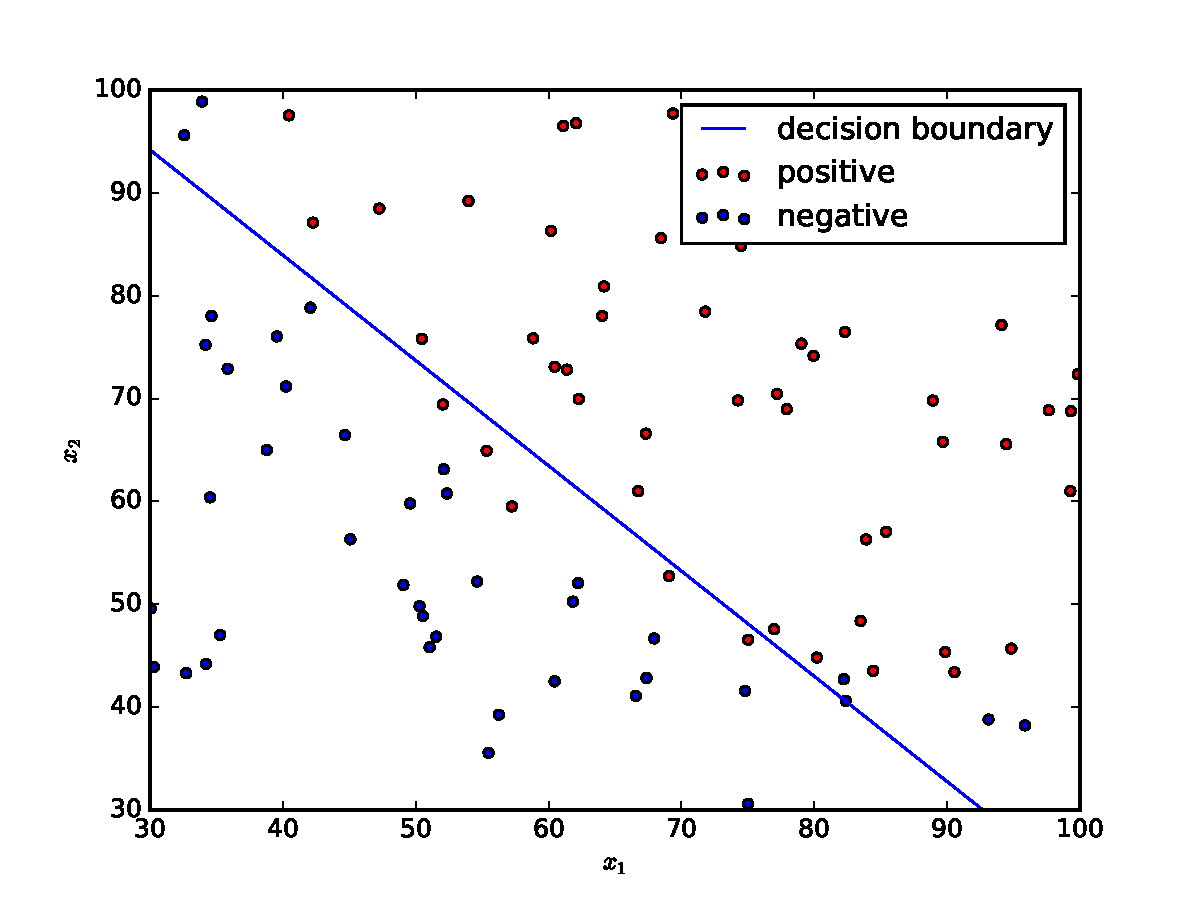
\includegraphics[width=0.85\textwidth]{ex2data1.pdf}
	\caption{线性决策边界}
\end{figure}

因此, 从另一个角度看, 进行 Logistic 回归, 实际上就是在求这个决策边界的回归方程, 或者说画一个超平面把两类点尽量地区分开来.

不过 Logistic 回归的威力不止于此, 如同线性回归一样, 它可以处理更复杂的模型, 比如对数据集 ex2data2.txt, 有
\begin{figure}[!htb]
	\centering
	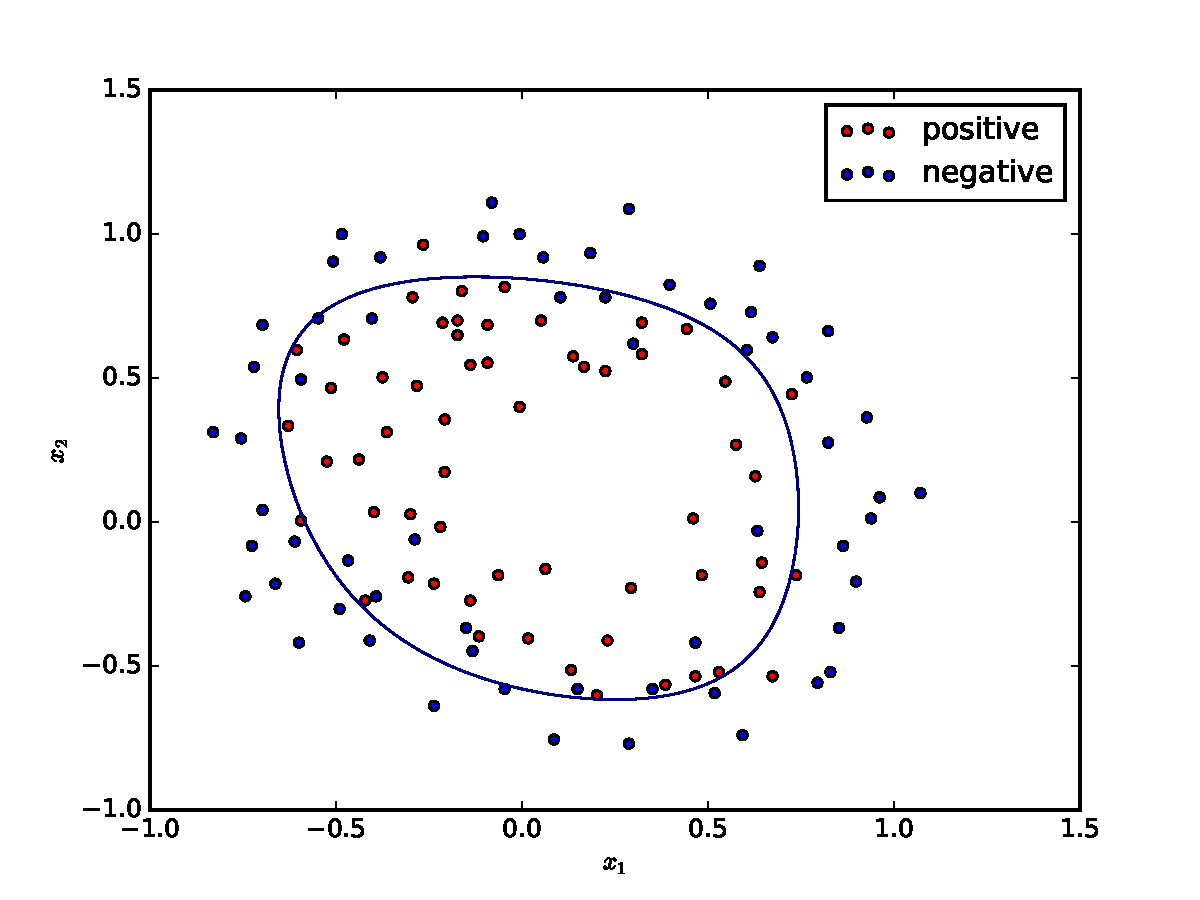
\includegraphics[width=0.85\textwidth]{ex2data2.pdf}
	\caption{非线性决策边界}
	\label{ex2data2}
\end{figure}

事实上, 如同线性回归一样, 模型看似是关于特征变量$x_{1}, x_{2}, \cdots, x_{n}$线性的, 这里“线性”的本质是关于参数$\theta_{0},\theta_{1},\cdots,\theta_{n}$的线性函数, 比如模型如果长这样:
\begin{equation*}
\theta_{0} + \theta_{1} x_{1}^{2} + \theta_{2} x_{1} x_{2} + \theta_{3} x_{2}^{4} + \theta_{4} x_{1}^{3} x_{2}^{3}
\end{equation*}

构造新的变量, 令
\begin{equation*}
z_{1} = x_{1}^{2}, z_{2} = x_{1} x_{2}, z_{3} = x_{2}^{4}, z_{4} = x_{1}^{3} x_{2}^{3}
\end{equation*}

则模型就变为了关于$\bm{z} = (z_{0},z_{1},\cdots,z_{4})^{T}$的线性模型了, 其中$z_{0} = 1$.
\begin{equation*}
\bm{\theta}^{T} \bm{z} = \theta_{0} + \theta_{1} z_{1} + \theta_{2}z_{2} + \theta_{3} z_{3} + \theta_{4} z_{4}
\end{equation*}

以数据集 ex2data2.txt 为例, 虽然只有$x_{1},x_{2}$两个特征, 但我们可以将其映射到一个高维空间中, 不妨将其称为 MapFeature, 假设映射到$6$次多项式, 即有
\begin{equation*}
\textrm{MapFeature}(\bm{x}) = (1, x_{1}, x_{2}, x_{1}^{2}, x_{1} x_{2}, x_{2}^{2}, \cdots, x_{2}^{6})
\end{equation*}

这样总共就有$1 + 2 + 3 + \cdots + 7 = 28$个特征, 于是可令$z_{0} = 1, z_{1} = x_{1}, \cdots, z_{28} = x_{2}^{6}$, 再应用 Logistic 回归模型即可, 求得回归参数$\theta_{0}, \theta_{1}, \cdots, \theta_{28}$以后, 决策边界的曲线方程为
\begin{equation*}
\theta_{0} + \theta_{1} x_{1} + \theta_{2} x_{2} + \theta_{3} x_{1}^{2} + \theta_{4} x_{1} x_{2} + \theta_{5} x_{2}^{2} + \cdots + \theta_{28} x_{2}^{6} = 0
\end{equation*}

这是一个隐函数的图像, 可以利用 ContourPlot 函数画出来.


模型越复杂, 相当于曲线越复杂, 理论上越能把两类点区分开来, 但是如同线性回归一样, 复杂的模型常常产生过拟合, 这就需要用下面的正则化来解决.


\section{正则化}

\subsection{过拟合与正则化}
Logistic 回归也有过拟合(overfitting)的问题, 一个复杂的模型可以保证训练误差非常小, 但是其测试误差和预测误差可能非常大, 这样模型就没有很好的预测能力. 为了防止过拟合, 我们通过施加惩罚项来解决这个问题. 如同线性回归一样, 参数$\bm{\theta}$反映了模型的复杂度, 因此可对参数$\bm{\theta}$施加惩罚, 比如, 代价函数为
\begin{equation*}
J(\bm{\theta}) = -\frac{1}{m} \sum_{i=1}^{m} \left[ y^{(i)} \log h_{\bm{\theta}}(\bm{x}^{(i)}) + (1 - y^{(i)}) \log (1 - h_{\bm{\theta}}(\bm{x}^{(i)})) \right] + \frac{\lambda}{2m} \sum_{j=1}^{n} \theta_{j}^{2}
\end{equation*}

注意我们不需要对$\theta_{0}$做惩罚, 所以上式右边的求和中$j$是从$1$到$n$, 而不是从$0$到$n$(虽然最后实际计算时差别影响不大). 同理可以求出导数为
\begin{align*}
\p{}{J(\bm{\theta})}{\theta_{0}} & = \frac{1}{m} \sum_{i=1}^{m} (h_{\bm{\theta}}(\bm{x}^{(i)}) - y^{(i)}) x_{j}^{(i)}  , & j = 0 \\
\p{}{J(\bm{\theta})}{\theta_{j}} & = \frac{1}{m} \left( \sum_{i=1}^{m} (h_{\bm{\theta}}(\bm{x}^{(i)}) - y^{(i)}) x_{j}^{(i)} + \lambda \theta_{j} \right)  , & j \geqslant 1
\end{align*}

\begin{figure}[!htb]
	\centering
	\subfigure[欠拟合]{
	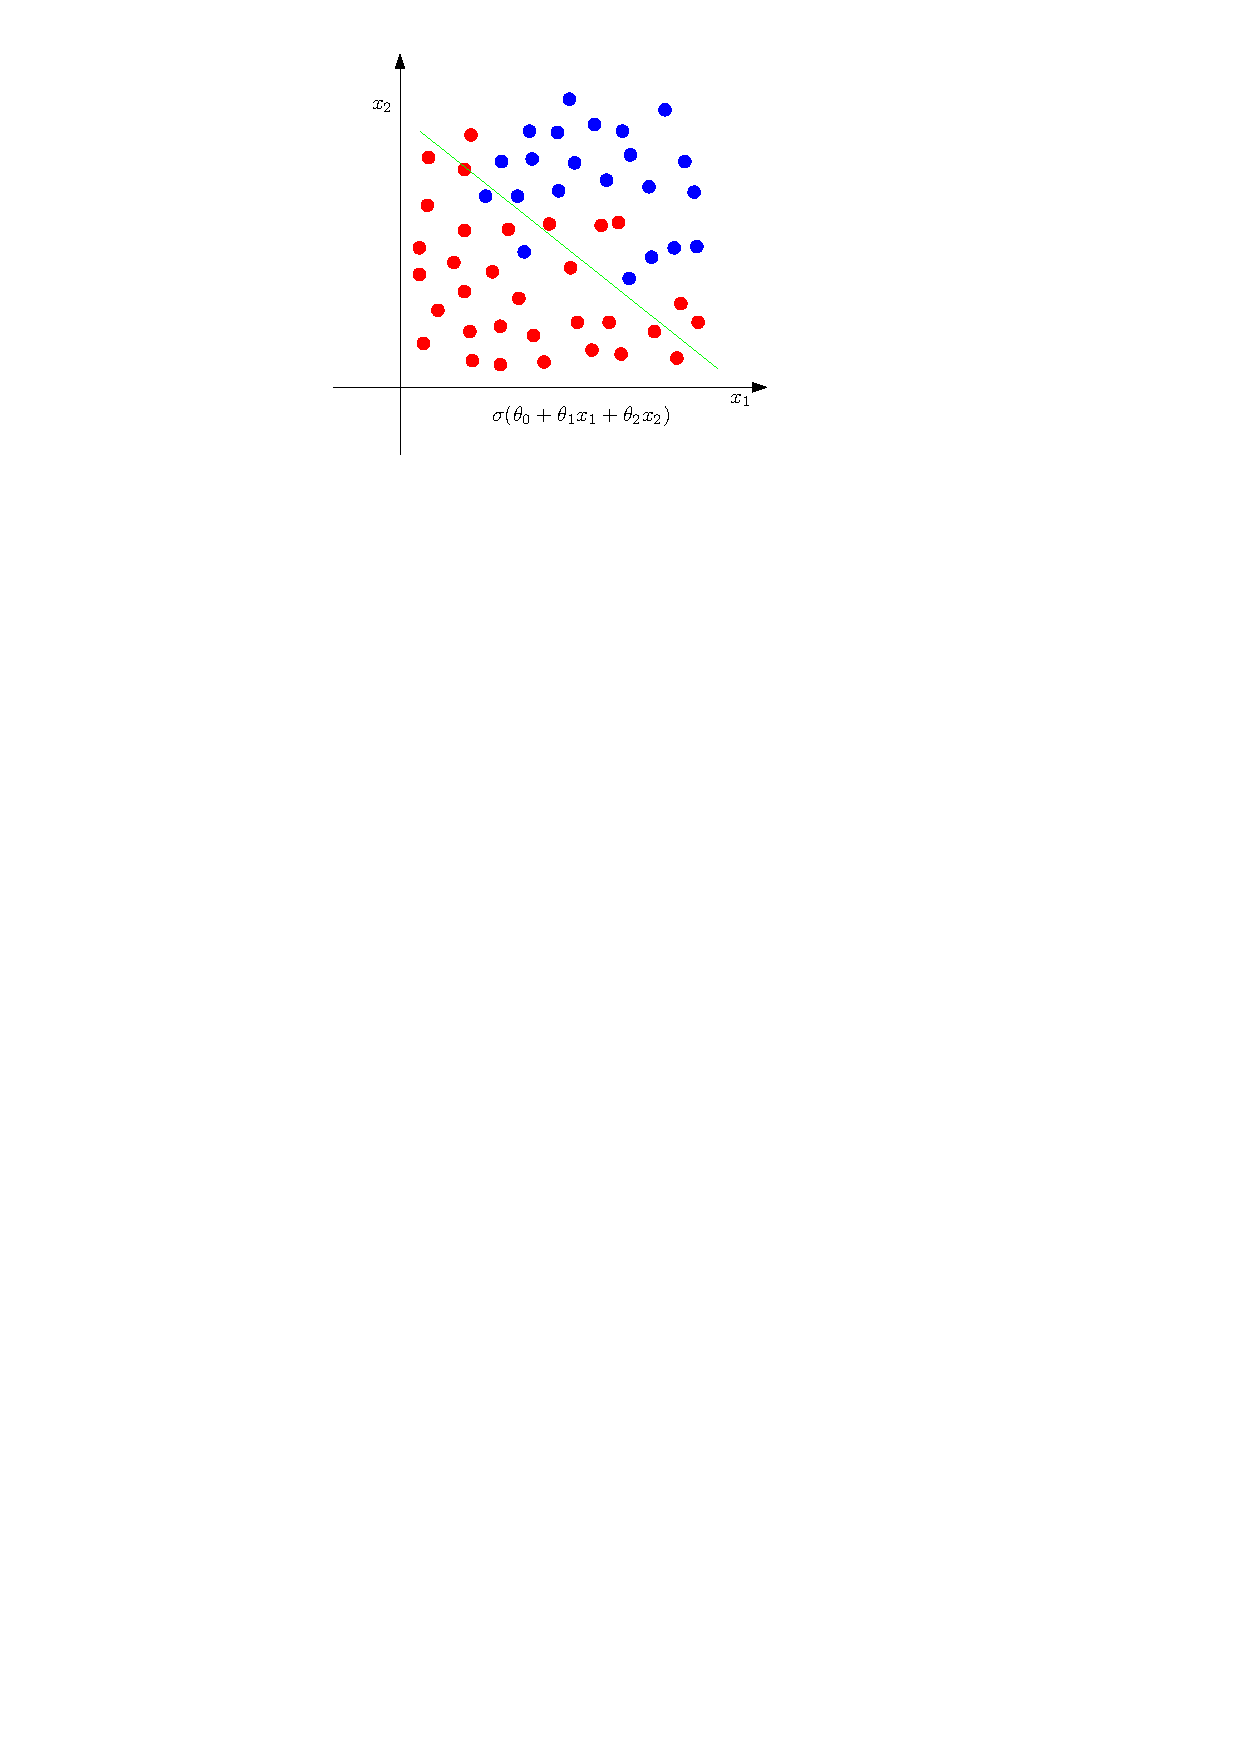
\includegraphics[width=1.2in]{fit1.pdf}
	}
	\hspace{0.3in}
	\subfigure[正常]{
	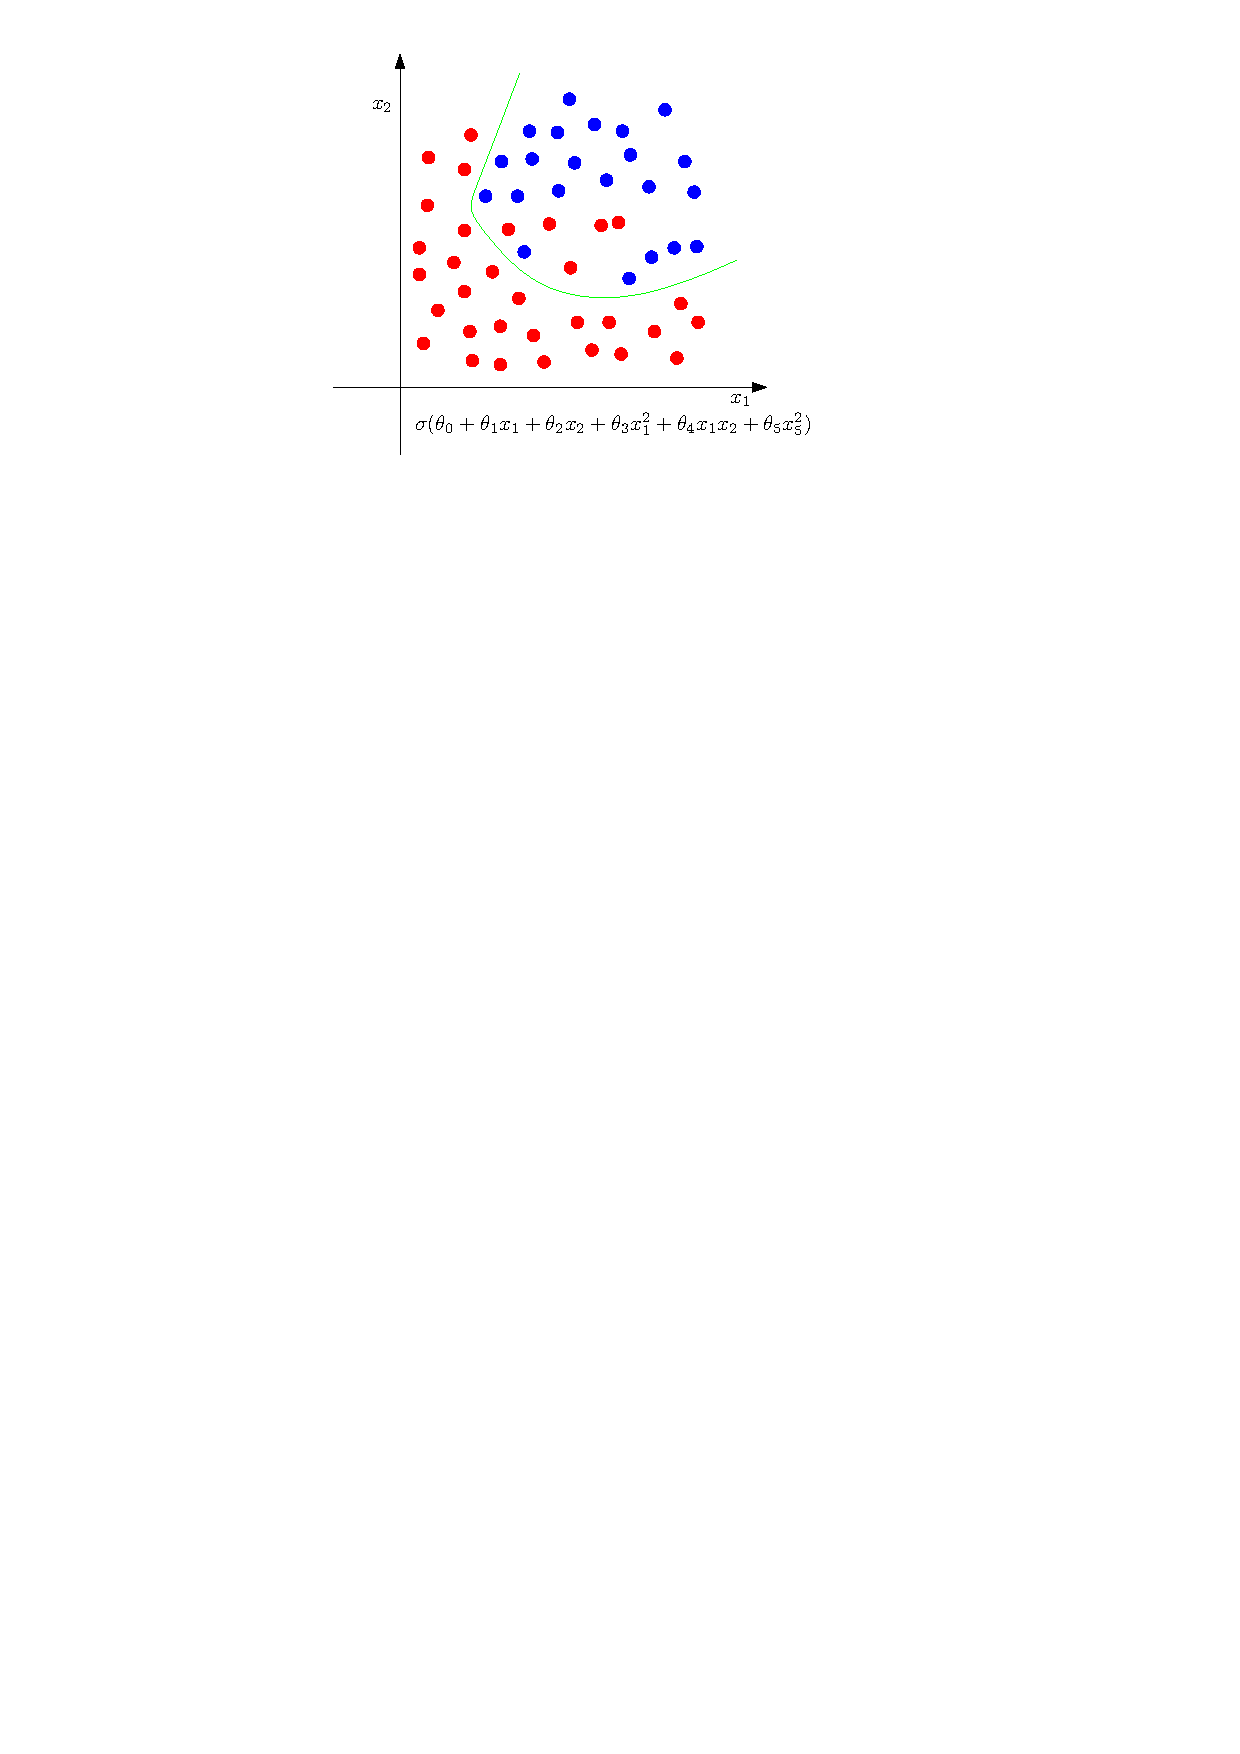
\includegraphics[width=1.2in]{fit2.pdf}
	}
	\hspace{0.3in}
	\subfigure[过拟合]{
	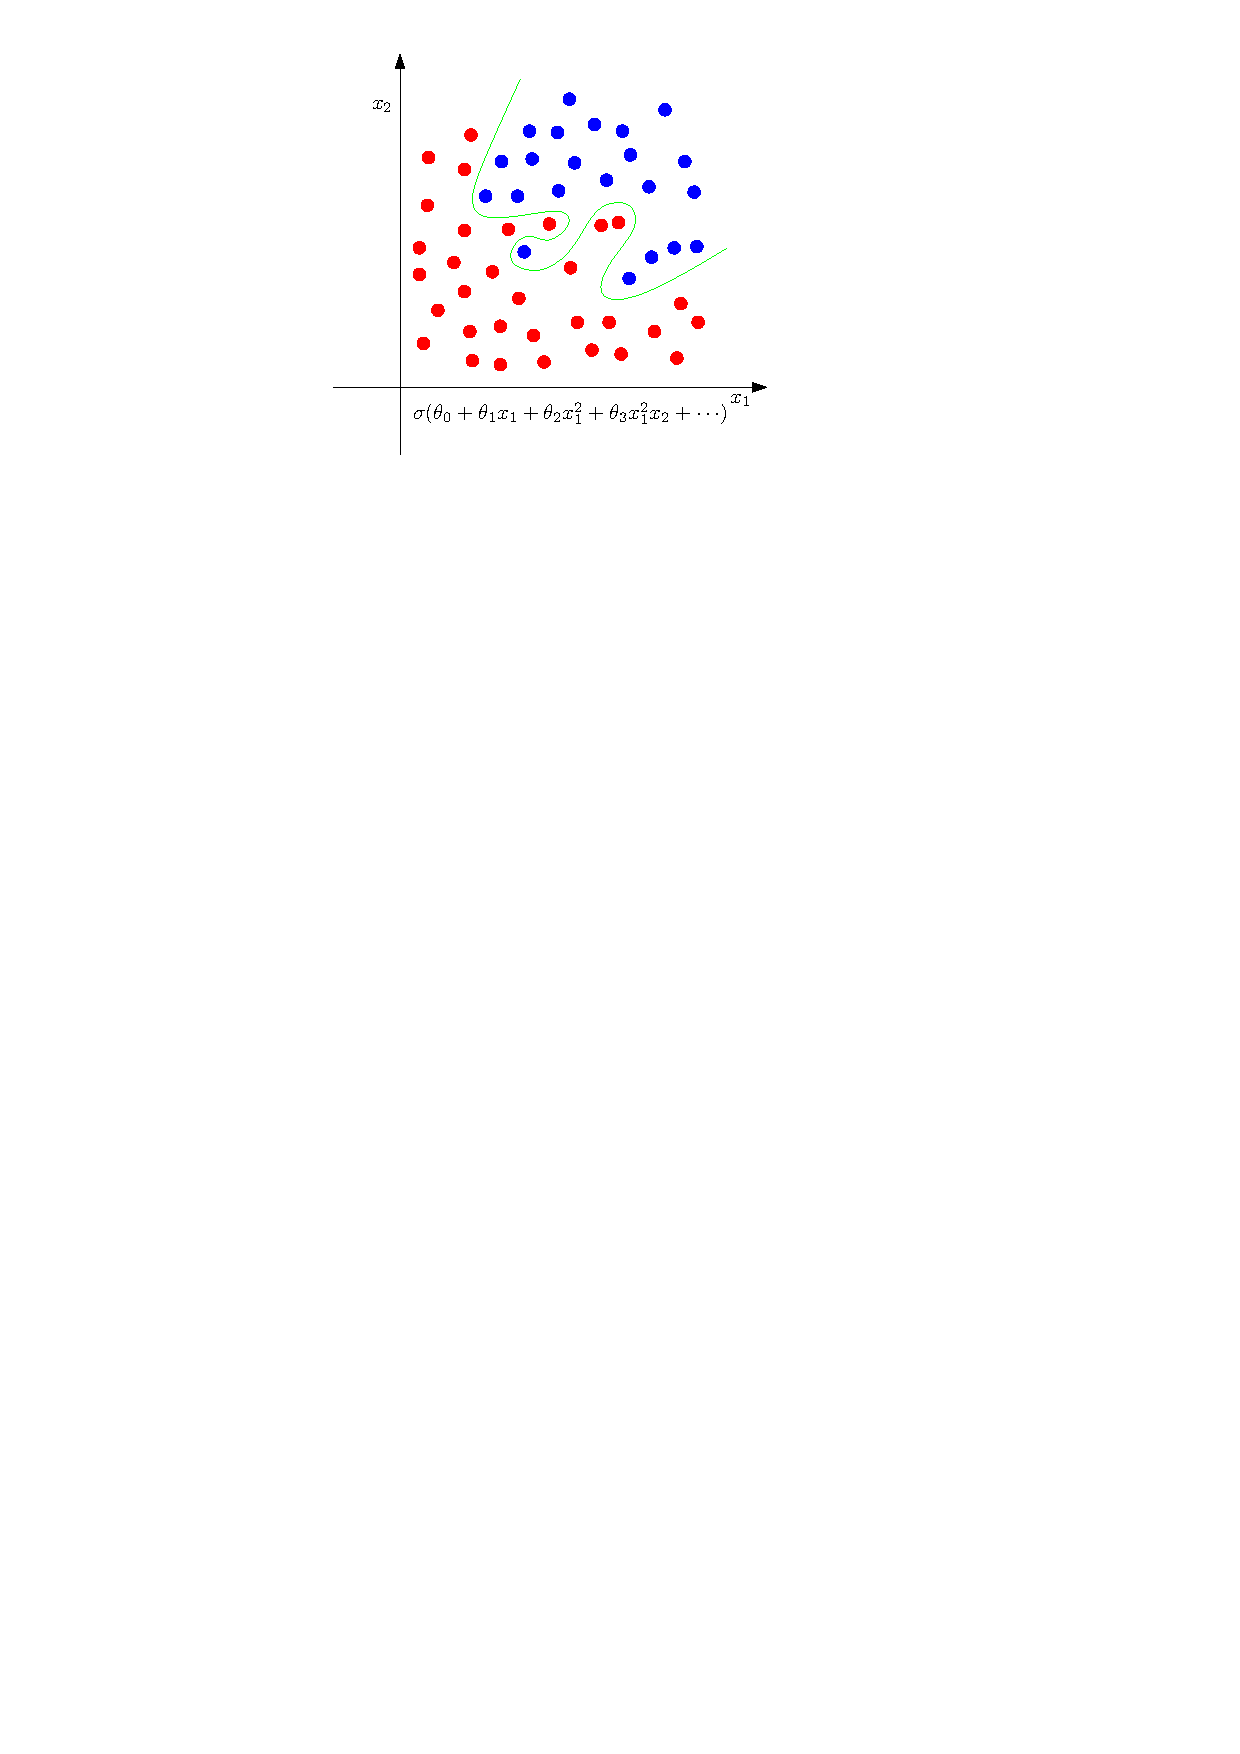
\includegraphics[width=1.2in]{fit3.pdf}
	}
	\caption{拟合情况}
	\label{logistic_fit}
\end{figure}

% \begin{figure}[!htb]
% 	\centering
% 	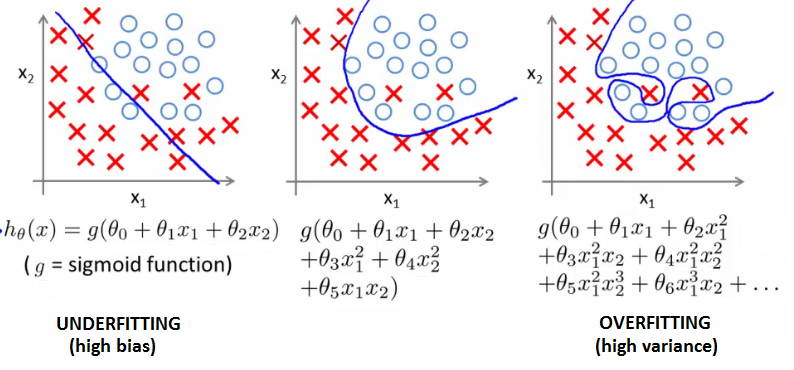
\includegraphics[width=0.80\textwidth]{overfit.png}
% 	\caption{拟合示意图}
% \end{figure}

前面提到过, 在未正则化时, 最大似然估计与构造代价函数本质上是一样的, 求得的参数估计均为
\begin{equation*}
\hat{\bm{\theta}} = \arg \min_{\bm{\theta}} \sum_{i=1}^{m} - \log p(y^{(i)} | \bm{x}^{(i)}; \bm{\theta})
\end{equation*}

略去常数因子, 我们上面对参数$\bm{\theta}$施加惩罚所得到的估计实际为
\begin{equation*}
\hat{\bm{\theta}} = \arg \min_{\bm{\theta}} \left( \sum_{i=1}^{m} - \log p(y^{(i)} | \bm{x}^{(i)}; \bm{\theta}) + \lambda ||\bm{\theta}||_{2} \right)
\end{equation*}

其中$||\bm{\theta}||_{2} = \sum\limits_{j=1}^{n} \theta_{j}^{2}$,求和指标$j$从1开始.

对数据集 ex2data2.txt 来说, 图\ref{ex2data2}正是用 MapFeature 结合正则化的方法画出来的.

也就是说, 上面实际上是$L_{2}$正则化, 当然, 我们也可以进行$L_{1}$正则化, 即有
\begin{equation*}
\hat{\bm{\theta}} = \arg \min_{\bm{\theta}} \left( \sum_{i=1}^{m} - \log p(y^{(i)} | \bm{x}^{(i)}; \bm{\theta}) + \lambda ||\bm{\theta}||_{1} \right)
\end{equation*}



\subsection{统计学角度看问题}
以上大都是从机器学习的角度来看问题, 主要的目的是估计出参数$\bm{\theta}$, 至于预测效果与模型选择等, 可由训练误差与测试误差决定.

大多数文献也都止步于此. 然而, 从经典统计学的角度看, 参数$\bm{\theta}$是一个未知的固定常数, 但是估计量$\hat{\bm{\theta}}$是一个随机变量, 是随机样本的函数, 因此, 也可以如同线性回归一样, 进一步分析估计量的统计性质, 比如分布等等, 进而寻求参数的区间估计, 或者对我们的结果进行假设检验, 比如模型系数的显著性检验, 以及利用 AIC 准则或者 BIC 准则进行模型选择等等. 这些确实也是可以做到的, 只不过不同与线性回归, 在 Logistic 回归中, 我们并没有得到估计量$\hat{\bm{\theta}}$的解析表达式, 因此进行这些工作会比较困难. 不过, 在  R语言和 Python 的 statmodels 包中, 可以给出相应的结果(注意在 Python 的 sklearn 包中, 是没有系数的显著性的).

另外一方面, 从贝叶斯统计的角度看, 一切未知量都是随机变量, 即参数$\bm{\theta}$不是一个未知的常数, 它也是一个随机变量, 只要我们给它一个合适的先验分布, 然后计算出后验分布, 也可进行各种统计推断, 而且往往比经典统计学更合理一些, 比如上面的最大似然估计会过拟合, 因此需要加上惩罚项来正则化, 而我们很容易证明, 假如$\bm{\theta}$的先验分布是 Laplace 分布, 即$p(\bm{\theta})  = (\lambda / 2)^{n} \exp (- \lambda ||\bm{\theta}||_{1})$, 其中常数$\lambda > 0$, 则$\bm{\theta}$的最大后验估计由下式给出:
\begin{equation*}
\min_{\bm{\theta}} \left( \sum_{i=1}^{m} - \log p(y^{(i)} | \bm{x}^{(i)}; \bm{\theta}) + \lambda ||\bm{\theta}||_{1} \right)
\end{equation*}

这恰好即为$L_{1}$正则化. 因此, 运用贝叶斯统计的观点来看问题, 能自动避免过拟合, 接下来我们就来看如何用贝叶斯方法进行 Logistic 回归.


\section{贝叶斯 Logistic 回归}
在贝叶斯统计中, 关键是要求出后验分布, 一般利用核方法, 即
\begin{equation*}
p(\bm{\theta} | \bm{x}) \propto p(\bm{\theta}) \cdot p(\bm{x} | \bm{\theta}) = p(\bm{\theta}) \cdot L(\bm{\theta} | \bm{x}) = K(\bm{\theta})
\end{equation*}

其中$L(\bm{\theta} | \bm{x})$就是样本似然函数$L(\bm{\theta})$, 最大后验估计即要使$K(\bm{\theta}) = p(\bm{\theta}) \cdot L(\bm{\theta | x})$最大. 注意在 Logistic 回归中, 这里的$p(\bm{\theta | x})$应当理解为$p(\bm{\theta | x}, y)$, 因为本质上$\bm{x}, y$合在一起是一组样本.

前面已经求得
\begin{equation*}
p(\bm{x} | \bm{\theta}) = L(\bm{\theta} | \bm{x}) = L(\bm{\theta}) = \prod_{i=1}^{m} p(y^{(i)} | \bm{x}^{(i)}; \bm{\theta})
\end{equation*}

下面来看$\bm{\theta}$的先验分布$p(\bm{\theta})$.

假定$\bm{\theta}$的先验分布为 Laplace 分布, 即
\begin{equation*}
p(\bm{\theta}) = \left(\frac{\lambda}{2} \right)^{n} \mathrm{e}^{-\lambda ||\bm{\theta}||_{1}}
\end{equation*}

其中$\lambda > 0$为常数, 则有
\begin{equation*}
K(\bm{\theta}) = p(\bm{\theta}) \cdot p(\bm{x} | \bm{\theta}) = \left(\frac{\lambda}{2} \right)^{n} \mathrm{e}^{-\lambda ||\bm{\theta}||_{1}} \cdot \prod_{i=1}^{m} p(y^{(i)} | \bm{x}^{(i)}; \bm{\theta})
\end{equation*}

对$K(\bm{\theta})$取负对数, 可得
\begin{equation*}
-\log K(\bm{\theta}) = - n \log \frac{\lambda}{2} + \lambda ||\bm{\theta}||_{1} - \sum_{i=1}^{m} \log p(y^{(i)} | \bm{x}^{(i)}; \bm{\theta})
\end{equation*}

极大化$K(\bm{\theta})$与极小化$- \log K(\bm{\theta})$是一样的, 即等价于
\begin{equation*}
\min_{\bm{\theta}} \left( \sum_{i=1}^{m} - \log p(y^{(i)} | \bm{x}^{(i)}; \bm{\theta}) + \lambda ||\bm{\theta}||_{1} \right)
\end{equation*}

这就是$L_{1}$正则化, 于是我们就得到了前面所说的结果.

此外, 如果假定$\bm{\theta}$的先验分布为
\begin{equation*}
\theta_{j} \sim \mathcal{N} (0, s^{2}) = \frac{1}{\sqrt{2 \pi} s} \mathrm{e}^{-\frac{\theta_{j}^{2}}{2s^2}} , j = 1, 2, \cdots, n
\end{equation*}

于是可得$\bm{\theta}$的先验分布为
\begin{equation*}
p(\bm{\theta}) = \prod_{j=1}^{n} \frac{1}{\sqrt{2 \pi} s} \mathrm{e}^{-\frac{\theta_{j}^{2}}{2s^2}} = \left( \frac{1}{\sqrt{2 \pi} s} \right)^{n} \mathrm{e}^{-\frac{\bm{\theta}^{T} \bm{\theta}}{2s^2}}
\end{equation*}

进一步有
\begin{equation*}
K(\bm{\theta}) = p(\bm{\theta}) \cdot p(\bm{x | \theta}) = \left( \frac{1}{\sqrt{2 \pi} s} \right)^{n} \mathrm{e}^{-\frac{\bm{\theta}^{T} \bm{\theta}}{2s^2}} \cdot \prod_{i=1}^{m} p(y^{(i)}|\bm{x}^{(i)};\bm{\theta})
\end{equation*}

还是对$K(\bm{\theta})$取负对数, 可得极小化$-\log K(\bm{\theta})$即为
\begin{equation*}
\min_{\bm{\theta}} \left( \sum_{i=1}^{m} - \log p(y^{(i)} | \bm{x}^{(i)}; \bm{\theta}) + \frac{\bm{\theta}^{T} \bm{\theta}}{2s^2} \right)
\end{equation*}

注意到$\bm{\theta}^{T} \bm{\theta} = ||\bm{\theta}||_{2}^{2}$, 因此这相当于$L^{2}$正则化.

以上正态分布的假定相当于$\bm{\theta} \sim \mathcal{N}(\bm{0}, s^{2}\bm{I})$. 当然, 我们也可以假定$\bm{\theta}$的先验分布为其他的形式, 比如$\bm{N(\mu, S)}$, 只不过处理会稍微复杂些, 这里就先不讨论了. 此外, 这里假定超参数比如$s$是已知的, 如果$s$未知, 我们也可以给$s$一个分布, 只不过讨论会更麻烦些.



\section{变分贝叶斯 Logistic 回归}

\subsection{变分贝叶斯一般框架}
在变分贝叶斯中, 我们将所有观测到的样本记为$\bm{X}$, 不妨设有$m$个样本, 即有$\bm{X} = \{ \bm{x}^{(1)}, \bm{x}^{(2)}, \cdots, \bm{x}^{(m)} \}$, 把所有的未知参数和隐变量(latent variable)记为$\bm{Z}$, 我们的目的是要估计出后验分布$p(\bm{Z} | \bm{X})$, 有了这个后验分布, 我们就可以估计出未知参数了.

但是解析的算出后验分布$p(\bm{Z} | \bm{X})$的表达式是几乎不可能的, 我们考虑用一个分布$q(\bm{Z})$去近似它. 为此先来看一个关系.
\begin{align*}
\ln p(\bm{X}) & = \ln \frac{p(\bm{X}, \bm{Z})}{p(\bm{Z} | \bm{X})}  = \int q(\bm{Z}) \ln \frac{p(\bm{X}, \bm{Z})}{p(\bm{Z} | \bm{X})} \diff \bm{Z} \\
& = \int q(\bm{Z}) \ln \left( \frac{p(\bm{X}, \bm{Z})}{p(\bm{Z} | \bm{X})} \cdot \frac{q(\bm{Z})}{q(\bm{Z})} \right) \diff \bm{Z} \\
& = \int q(\bm{Z}) \left( \ln \frac{q(\bm{Z})}{p(\bm{Z} | \bm{X})} + \ln \frac{p(\bm{X}, \bm{Z})}{q(\bm{Z})} \right) \diff \bm{Z} \\
& = \int q(\bm{Z}) \cdot \ln \frac{q(\bm{Z})}{p(\bm{Z} | \bm{X})} \diff \bm{Z} + \int q(\bm{Z}) \cdot \ln \frac{p(\bm{X}, \bm{Z})}{q(\bm{Z})} \diff \bm{Z} \\
& = - \int q(\bm{Z}) \cdot \ln \frac{p(\bm{Z} | \bm{X})}{q(\bm{Z})} \diff \bm{Z} + \int q(\bm{Z}) \cdot \ln \frac{p(\bm{X}, \bm{Z})}{q(\bm{Z})} \diff \bm{Z} \\
& = \mathrm{KL}(q||p) + \mathcal{L}(q)
\end{align*}

其中$\mathrm{KL}(q || p)$表示$q(\bm{Z})$与$p(\bm{Z} | \bm{X})$间的 KL 散度.
\begin{equation*}
\mathrm{KL}(q || p) = - \int q(\bm{Z}) \cdot \ln \frac{p(\bm{Z} | \bm{X})}{q(\bm{Z})} \diff \bm{Z} \geqslant 0
\end{equation*}

从这个角度看, $\mathrm{KL}(q || p)$反映了我们用$q(\bm{Z})$去近似$p(\bm{Z} | \bm{X})$的差距, 这个值越小越好, 而且我们知道$\mathrm{KL}(q || p) = 0 \Longleftrightarrow q(\bm{Z}) = p(\bm{Z} | \bm{X})$.

在这里, 我们是通过不断最大化$\mathcal{L}(q)$来达到相同的目的, 而$\mathcal{L}(q)$刚好是一个函数$q(\bm{Z})$的泛函, 变分的名称由此得来.

如同一般的变分法, 这里要对$q(\bm{Z})$做某些要求, 相当于把$q(\bm{Z})$限制到某个空间中. 假设$\bm{Z}$可独立成$M$个部分$Z_{i}, i = 1,2,\cdots,M$, 那么最常用的一个要求是因子分解分布, 即有
\begin{equation*}
q(\bm{Z}) = \prod_{i=1}^{M} q_{i}(Z_{i})
\end{equation*}

在此限定条件下我们来求$\mathcal{L}(q)$的最大值, 总体思路是把$\mathcal{L}(q)$拆分成独立的$q_{j}(Z_{j})$, 从而对每一项求最大值, 以下推导中将$q_{j}(Z_{j})$简记为$q_{j}$, 于是有
\begin{align*}
\mathcal{L}(q) & = \int q(\bm{Z}) \cdot \ln \frac{p(\bm{X}, \bm{Z})}{q(\bm{Z})} \diff \bm{Z} \\
& = \int \prod_{i} q_{i}(Z_{i}) \left( \ln p(\bm{X}, \bm{Z}) - \ln \prod_{i}q_{i}(Z_{i}) \right) \diff \bm{Z} \\
& = \int \prod_{i} q_{i} \left( \ln p(\bm{X}, \bm{Z}) - \sum_{i} \ln q_{i} \right) \diff \bm{Z} \\
& = \int \prod_{i} q_{i} \ln p(\bm{X}, \bm{Z}) \prod_{i} \diff Z_{i} - \sum_{i} \int \prod_{j} q_{j} \ln q_{i} \diff Z_{i} \\
& = \int q_{j} \left( \ln p(\bm{X}, \bm{Z}) \prod_{i \neq j} (q_{i} \diff Z_{i}) \right) \diff Z_{j} - \int q_{j} \ln q_{j} \diff Z_{j} - \sum_{i \neq j} \int q_{i} \ln q_{i} \diff Z_{i} \\
& = \int q_{j} \ln \tilde{p}(\bm{X},Z_{j}) \diff Z_{j} - \int q_{j} \ln q_{j} \diff Z_{j} - \sum_{i \neq j} \int q_{i} \ln q_{i} \diff Z_{i} \\
& = - \int q_{j} \ln \frac{\tilde{p}(\bm{X},Z_{j})}{q_{j}} \diff Z_{j} - \sum_{i \neq j} \int q_{i} \ln q_{i} \diff Z_{i} \\
& = - \mathrm{KL}(q_{j} || \tilde{p}) - \sum_{i \neq j} \int q_{i} \ln q_{i} \diff Z_{i}
\end{align*}

其中
\begin{equation*}
\ln \tilde{p}(\bm{X}, Z_{j}) = \int \ln p(\bm{X}, \bm{Z}) \prod_{i \neq j} (q_{i} \diff Z_{i}) = \mathbb{E}_{i \neq j}[\ln p(\bm{X}, \bm{Z})]
\end{equation*}

显然, 当$\mathrm{KL}(q_{j} || \tilde{p}) = 0$时上式取得最大值, 也即$q_{j}(Z_{j}) = \tilde{p}(\bm{X}, Z_{j})$, 因此最优分布$q_{j}^{*}(Z_{j})$即为
\begin{equation*}
\ln q_{j}^{*}(Z_{j}) = \ln \tilde{p}(\bm{X}, Z_{j}) = \mathbb{E}_{i \neq j}[\ln p(\bm{X}, \bm{Z})] + \textrm{const}
\end{equation*}

这里的常数是为了保证分布$q_{j}^{*}(Z_{j})$的正则性, 直接进行归一化可得
\begin{equation*}
q_{j}^{*}(Z_{j}) = \frac{\exp(\mathbb{E}_{i \neq j}[\ln p(\bm{X}, \bm{Z})])}{\displaystyle \int \mathrm{exp}(\mathbb{E}_{i \neq j}[\ln p(\bm{X}, \bm{Z})]) \diff Z_{j}}
\end{equation*}

这便是最优分布的表达式.

关于变分贝叶斯还有很多东西, 这里就不再讨论了.


\subsection{变分贝叶斯Logistic回归}
现在, 我们来运用变分贝叶斯方法进行 Logistic 回归.

\begin{remark}
这里推导的结果的表达式仍然是以类标签$y$取值为$1$或$0$的, 这与 PRML 上保持的是一致的, 不过推导结果是借鉴的 Jan Drugowitsch 的文献, 文献上用的类标签是$\pm 1$, 不过仔细推导可以发现, 二者其实也是一致的, 在得出$h(\bm{\theta}, \bm{\xi})$的时候其表达式实质上就是相同的. 事实上, 如果用$y = 1, 0$作为类标签, 那么转化关系$y^{*} = 2 \cdot y - 1$, 就将$y^{*}$化为了$\pm 1$.

\end{remark}

设参数$\bm{\theta}$的先验分布为依赖于超参数$\alpha$的正态分布, 即$\bm{\theta}\sim \mathcal{N}(\bm{0}, \alpha^{-1} \bm{I})$
\begin{equation*}
p(\bm{\theta} | \alpha) = \left( \frac{\alpha}{2 \pi}\right)^{n/2} \mathrm{exp} \left( -\frac{\alpha}{2} \bm{\theta}^{T} \bm{\theta} \right)
\end{equation*}

而$\alpha$服从伽马分布$\alpha \sim \mathrm{Gam}(a_{0}, b_{0})$, 即有
\begin{equation*}
p(\alpha) = \frac{1}{\Gamma(a_0)} b_{0}^{a_0} \alpha^{a_{0} - 1} \mathrm{exp}(- b_{0} \alpha)
\end{equation*}

我们的目的是用一个分布$q(\bm{\theta}, \alpha)$去近似后验分布, 首先假设$q(\bm{\theta}, \alpha) = q(\bm{\theta}) q(\alpha)$, 不过将变分贝叶斯运用到 Logistic 回归中还是会有些困难, 接下来将直接给出结果. 可以求得

\begin{align*}
\ln q^{*}(\bm{\theta}) & = \bm{\theta}^{T} \sum_{i} \frac{2 y^{(i)} - 1}{2} \bm{x}^{(i)} - \frac{1}{2} \bm{\theta}^{T} \left( \mathbb{E}_{\alpha}(\alpha) \bm{I} + 2 \sum_{i} \lambda(\xi_{i}) \bm{x}^{(i)} (\bm{x}^{(i)})^{T} \right) \bm{\theta} + \mathrm{const} \\ 
& = \ln \mathcal{N}(\bm{\theta} | \bm{\theta}_{m},\bm{S}_{m})
\end{align*}

其中
\begin{align*}
\bm{S}_{m}^{-1} & = \mathbb{E}_{\alpha}(\alpha) \bm{I} + 2 \sum_{i} \lambda(\xi_{i}) \bm{x}^{(i)} (\bm{x}^{(i)})^{T} \\
\bm{\theta}_{m} & = \bm{S}_{m} \sum_{i} \frac{2 y^{(i)} - 1}{2} \bm{x}^{(i)} \\
\lambda(\xi) & = \frac{1}{2 \xi} \left( \sigma(\xi) - \frac{1}{2} \right)
\end{align*}

类似地, 对于$\alpha$有
\begin{align*}
\ln q^{*}(\alpha) & = \left( a_{0} - 1 + \frac{n}{2} \right) \ln \alpha - \left( b_{0} + \frac{1}{2} \mathbb{E}_{\bm{\theta}}(\bm{\theta}^{T} \bm{\theta}) \right) \alpha + \mathrm{const} \\
& = \ln \mathrm{Gam}(\alpha | a_{m}, b_{m})
\end{align*}

其中
\begin{equation*}
a_{m} = a_{0} + \frac{n}{2}  \qquad b_{m} = b_{0} + \frac{1}{2}\mathbb{E}_{\bm{\theta}}(\bm{\theta}^{T} \bm{\theta})
\end{equation*}

上述公式中的期望可由下式计算
\begin{equation*}
\mathbb{E}_{\alpha}(\alpha) = \frac{a_{m}}{b_{m}}  \qquad  \mathbb{E}_{\bm{\theta}}(\bm{\theta}^{T} \bm{\theta}) = \bm{\theta}_{m}^{T} \bm{\theta}_{m} + \mathrm{Tr}(\bm{S}_{m})
\end{equation*}

可以看到, 不管是计算$\bm{\theta}$还是$\alpha$都要依赖地用到对方的信息, 因此可用 EM 算法来进行计算, 其中$\xi$的更新过程为
\begin{equation*}
\xi_{i}^{\mathrm{new}} = \sqrt{(\bm{x}^{(i)})^{T} (\bm{S}_{m} + \bm{\theta}_{m} \bm{\theta}_{m}^{T}) \bm{x}^{(i)}}
\end{equation*}

最终由 EM 算法即可算得参数$\bm{\theta}$的值. 此外, 运用变分贝叶斯还可以直接对概率分布作预测, 这里也就不再讨论了.



\section{总结}

\subsection{参考资料}

\begin{enumerate}[(1)]
\item 博客: \url{http://aimotion.blogspot.lt/2011/11/machine-learning-with-python-logistic.html}, 有 Python 编程, 但是原理推导不够详细.
\item 博客: \url{https://www.kunxi.org/notes/Machine_Learning/Logistic_Regression/}, 有 Python 编程和部分原理推导
\item R-bloggers: \url{http://www.r-bloggers.com/interactive-visualization-of-non-linear-logistic-regression-decision-boundaries-with-shiny/} 一个交互式绘出决策边界的 R 语言实现
\item StackOverflow: \url{http://stackoverflow.com/questions/22294241/plotting-a-decision-boundary-separating-2-classes-using-matplotlibs-pyplot} 运用 sklearn 画出决策边界
\item R-bloggers: \url{http://www.r-bloggers.com/machine-learning-ex-5-2-regularized-logistic-regression/} 正则化 Logistic 回归的 R 实现
\item CSDN: \url{http://blog.csdn.net/dongtingzhizi/article/details/15962797} 推导很详细
\item CSDN: \url{http://blog.csdn.net/zouxy09/article/details/20319673} 写的较为通俗
\item 公开课材料: \url{http://openclassroom.stanford.edu/MainFolder/DocumentPage.php?course=MachineLearning&doc=exercises/ex5/ex5.html} Matlab 代码实现
\end{enumerate}





\newpage

\section*{附录}





\end{document}